% Propósito: enseñar la convención de lectura de un audiograma y mostrar que
% la diferencia entre vía aérea y vía ósea se calcula frecuencia por frecuencia.
% Origen: definición de G_AO(f) en \eqref{eq:u8-gap}. Los seis pares de puntos
% son datos didácticos ficticios, no mediciones, normas ni patrones diagnósticos.
% Las frecuencias de octava se ubican a distancias iguales, equivalentes a un
% eje logarítmico de base 2. En 1000 Hz se reproducen los valores del ejemplo
% del texto: 40 dB HL por vía aérea y 15 dB HL por vía ósea.
% Descripción accesible: el eje horizontal muestra frecuencias entre 250 y
% 8000 Hz en posiciones de octava. El eje vertical muestra nivel de audición
% en dB HL y aumenta hacia abajo según la convención audiométrica. Dos trazos
% ficticios representan vía aérea y vía ósea. En 1000 Hz una flecha vertical
% marca una diferencia de 25 dB, sin atribuirle diagnóstico.
% Validación prevista: comprobar el sentido del eje vertical, las etiquetas y
% unidades, la separación entre rótulo y números del eje vertical, la posición
% de las frecuencias sobre el eje, la resta 40 dB HL - 15 dB HL = 25 dB y la
% legibilidad en página.
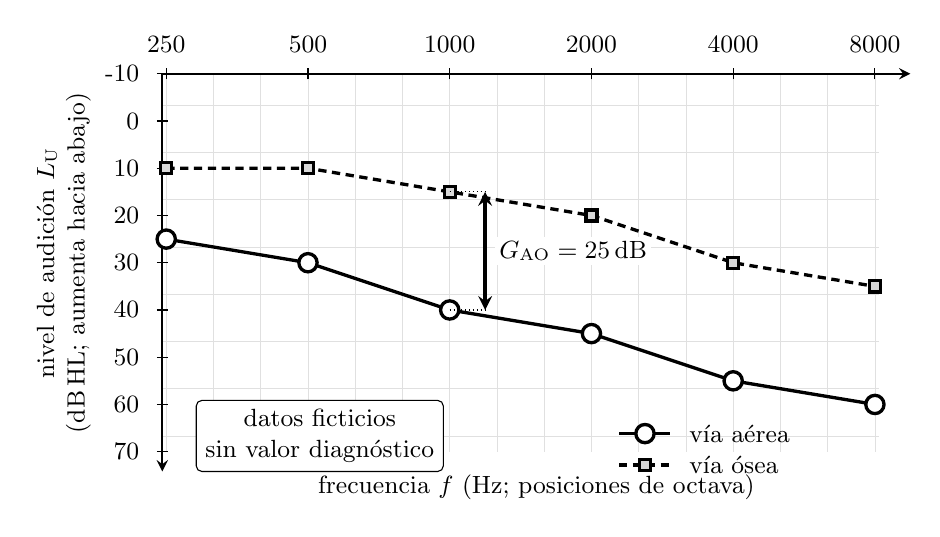
\begin{tikzpicture}[font=\small,>=stealth,x=1cm,y=1cm]
    \draw[step=0.60cm,black!12,very thin] (1.15,0.40) grid (10.25,5.20);

    \draw[->,thick] (1.15,5.20) -- (1.15,0.15);
    \draw[->,thick] (1.15,5.20) -- (10.65,5.20);
    \node[rotate=90,align=center] at (-0.10,2.80)
        {nivel de audición \(L_\mathrm{U}\)\\(\(\mathrm{dB\,HL}\); aumenta hacia abajo)};
    \node[align=center] at (5.90,-0.05)
        {frecuencia \(f\) (\(\mathrm{Hz}\); posiciones de octava)};

    \foreach \y/\lab in {
        5.20/-10,4.60/0,4.00/10,3.40/20,2.80/30,
        2.20/40,1.60/50,1.00/60,0.40/70}{
        \draw (1.08,\y) -- (1.22,\y);
        \node[anchor=east] at (0.98,\y) {\lab};
    }

    \foreach \x/\lab in {
        1.20/250,3.00/500,4.80/1000,6.60/2000,8.40/4000,10.20/8000}{
        \draw (\x,5.13) -- (\x,5.27);
        \node[anchor=south] at (\x,5.34) {\lab};
    }

    % Vía aérea ficticia: 25, 30, 40, 45, 55 y 60 dB HL.
    \draw[very thick]
        plot coordinates {
            (1.20,3.10) (3.00,2.80) (4.80,2.20)
            (6.60,1.90) (8.40,1.30) (10.20,1.00)
        };
    \foreach \x/\y in {
        1.20/3.10,3.00/2.80,4.80/2.20,
        6.60/1.90,8.40/1.30,10.20/1.00}{
        \draw[very thick,fill=white] (\x,\y) circle (3.3pt);
    }

    % Vía ósea ficticia: 10, 10, 15, 20, 30 y 35 dB HL.
    \draw[very thick,densely dashed]
        plot coordinates {
            (1.20,4.00) (3.00,4.00) (4.80,3.70)
            (6.60,3.40) (8.40,2.80) (10.20,2.50)
        };
    \foreach \x/\y in {
        1.20/4.00,3.00/4.00,4.80/3.70,
        6.60/3.40,8.40/2.80,10.20/2.50}{
        \draw[very thick,fill=black!15] (\x-0.07,\y-0.07) rectangle ++(0.14,0.14);
    }

    \draw[densely dotted] (4.80,2.20) -- (5.25,2.20);
    \draw[densely dotted] (4.80,3.70) -- (5.25,3.70);
    \draw[<->,very thick] (5.25,2.20) -- (5.25,3.70)
        node[midway,right=3pt,fill=white,inner sep=1.5pt]
        {\(G_{\mathrm{AO}}=25\,\mathrm{dB}\)};

    \draw[very thick] (6.95,0.63) -- (7.60,0.63);
    \draw[very thick,fill=white] (7.28,0.63) circle (3.3pt);
    \node[anchor=west] at (7.72,0.63) {vía aérea};
    \draw[very thick,densely dashed] (6.95,0.23) -- (7.60,0.23);
    \draw[very thick,fill=black!15] (7.21,0.16) rectangle ++(0.14,0.14);
    \node[anchor=west] at (7.72,0.23) {vía ósea};

    \node[draw,rounded corners=2pt,fill=white,align=center]
        at (3.15,0.60)
        {datos ficticios\\sin valor diagnóstico};
\end{tikzpicture}
